\chapter{Proposition d'une nouvelle famille virale associée aux Hyménoptères parasitoïdes}

Dans le chapitre précédent (\hyperref[sec:chap1]{chapitre 1}), nous avons cherché la présence d'éléments viraux endogénisés (EVEs) dans le génome de nombreuses espèces d'Hyménoptères. Le pipeline développé pour cet usage, nous a également permis d'observer la présence de plusieurs éléments viraux exogènes appartenant probablement à des virus à ADN libres séquencés au même moment que les génomes des insectes (pour plus d'informations sur ces éléments exogènes, veuillez vous référer à la section \hyperref[sec:perspective]{perspective} du manuscrit de thèse). Ces nouveaux scaffolds nous ont donné l'opportunité de décrire de nouveaux virus, dont certains ont été retrouvés chez des espèces parasitoïdes. De manière intéressante, certains de ces virus étaient apparentés à un virus qui était jusque-là le seul représentant d'une probable nouvelle famille de virus à ADN double brin \citep{lepetit_genome_2017}. Ce virus se nomme Leptopilina boulardi filamentous virus (LbFV) et infecte comme son nom l'indique le parasitoïde de drosophiles \textit{Leptopilina boulardi}. Bien que son mode de transmission majoritaire soit vertical, ce virus induit un changement de comportement de ponte favorisant une transmission horizontale en situation de superparasitisme (ponte dans un œuf déjà parasité). En effet, les femelles infectées acceptent de pondre dans des hôtes déjà parasités beaucoup plus fréquemment que les femelles non-infectées, favorisant ainsi la transmission horizontale du virus \citep{varaldi_infectious_2003}. Cette manipulation du comportement permet ainsi au virus de se propager plus efficacement au sein des populations de parasitoïdes. En analysant les 124 génomes d'Hyménoptères décrits dans le chapitre précédent, j'ai pu obtenir la séquence complète ou quasi complète de 4 génomes supplémentaires de virus apparentés à LbFV. En parallèle, l’équipe de l’IRBI de Tours faisait également des découvertes connexes chez des virus filamenteux apparentés au sein du génome de \textit{Cotesia congregata} avec la présence de 2 souches (CcFV1 et CcFV2) dont les génomes complets ont été assemblés. \\

Dans cette deuxième étude, nous caractérisons ainsi six nouveaux génomes viraux apparentés à LbFV. Ils proviennent tous de guêpes parasitoïdes: \textit{Leptopilina heterotoma} (Cynipoidea, Figitidae), \textit{Encarsia formosa} (Chalcidoidea, Aphelinidae), \textit{Platygaster orseoliae} (Platygastroidea, Platygastridae), \textit{Psyttalia concolor}, et deux souches de \textit{Cotesia congregata}  (Ichneumonoidea, Braconidae). Grâce à de la génomique comparative et des analyses phylogénétiques approfondies de ces génomes, ainsi qu'à une étude de la morphogenèse des particules, nous étudions la possibilité que ces "virus filamenteux" représentent une nouvelle famille virale au sein des \textit{Naldaviricetes}. Nous démontrons que ces virus filamenteux partagent des caractéristiques morphologiques, génomiques et phylogénétiques qui les distinguent de leurs plus proches parents, les \textit{Hytrosaviridae}. \\

Nous décrivons ainsi la présence de tous les gènes cœurs essentiels au fonctionnement des virus de la classe des \textit{Naldaviricetes} (\figurename{\ref{figure:Resume_figure_papier2}}-A). Mais de manière plus intéressante, nous décrivons également la présence de 5 gènes partagés par tous les membres de cette possible nouvelle famille virale et qui leur sont spécifiques (\figurename{\ref{figure:Resume_figure_papier2}}-A, en bleu). Bien que nous n'ayons par d'idée précise sur la fonction de ces gènes, le fait qu'ils soient présents systématiquement chez tous les virus filamenteux étudiés soutient l'hypothèse qu'ils ont d'importantes fonctions partagées par tous ces virus. \\


\begin{figure}[!htpbt]
\captionsetup{font=footnotesize}
 \centering
  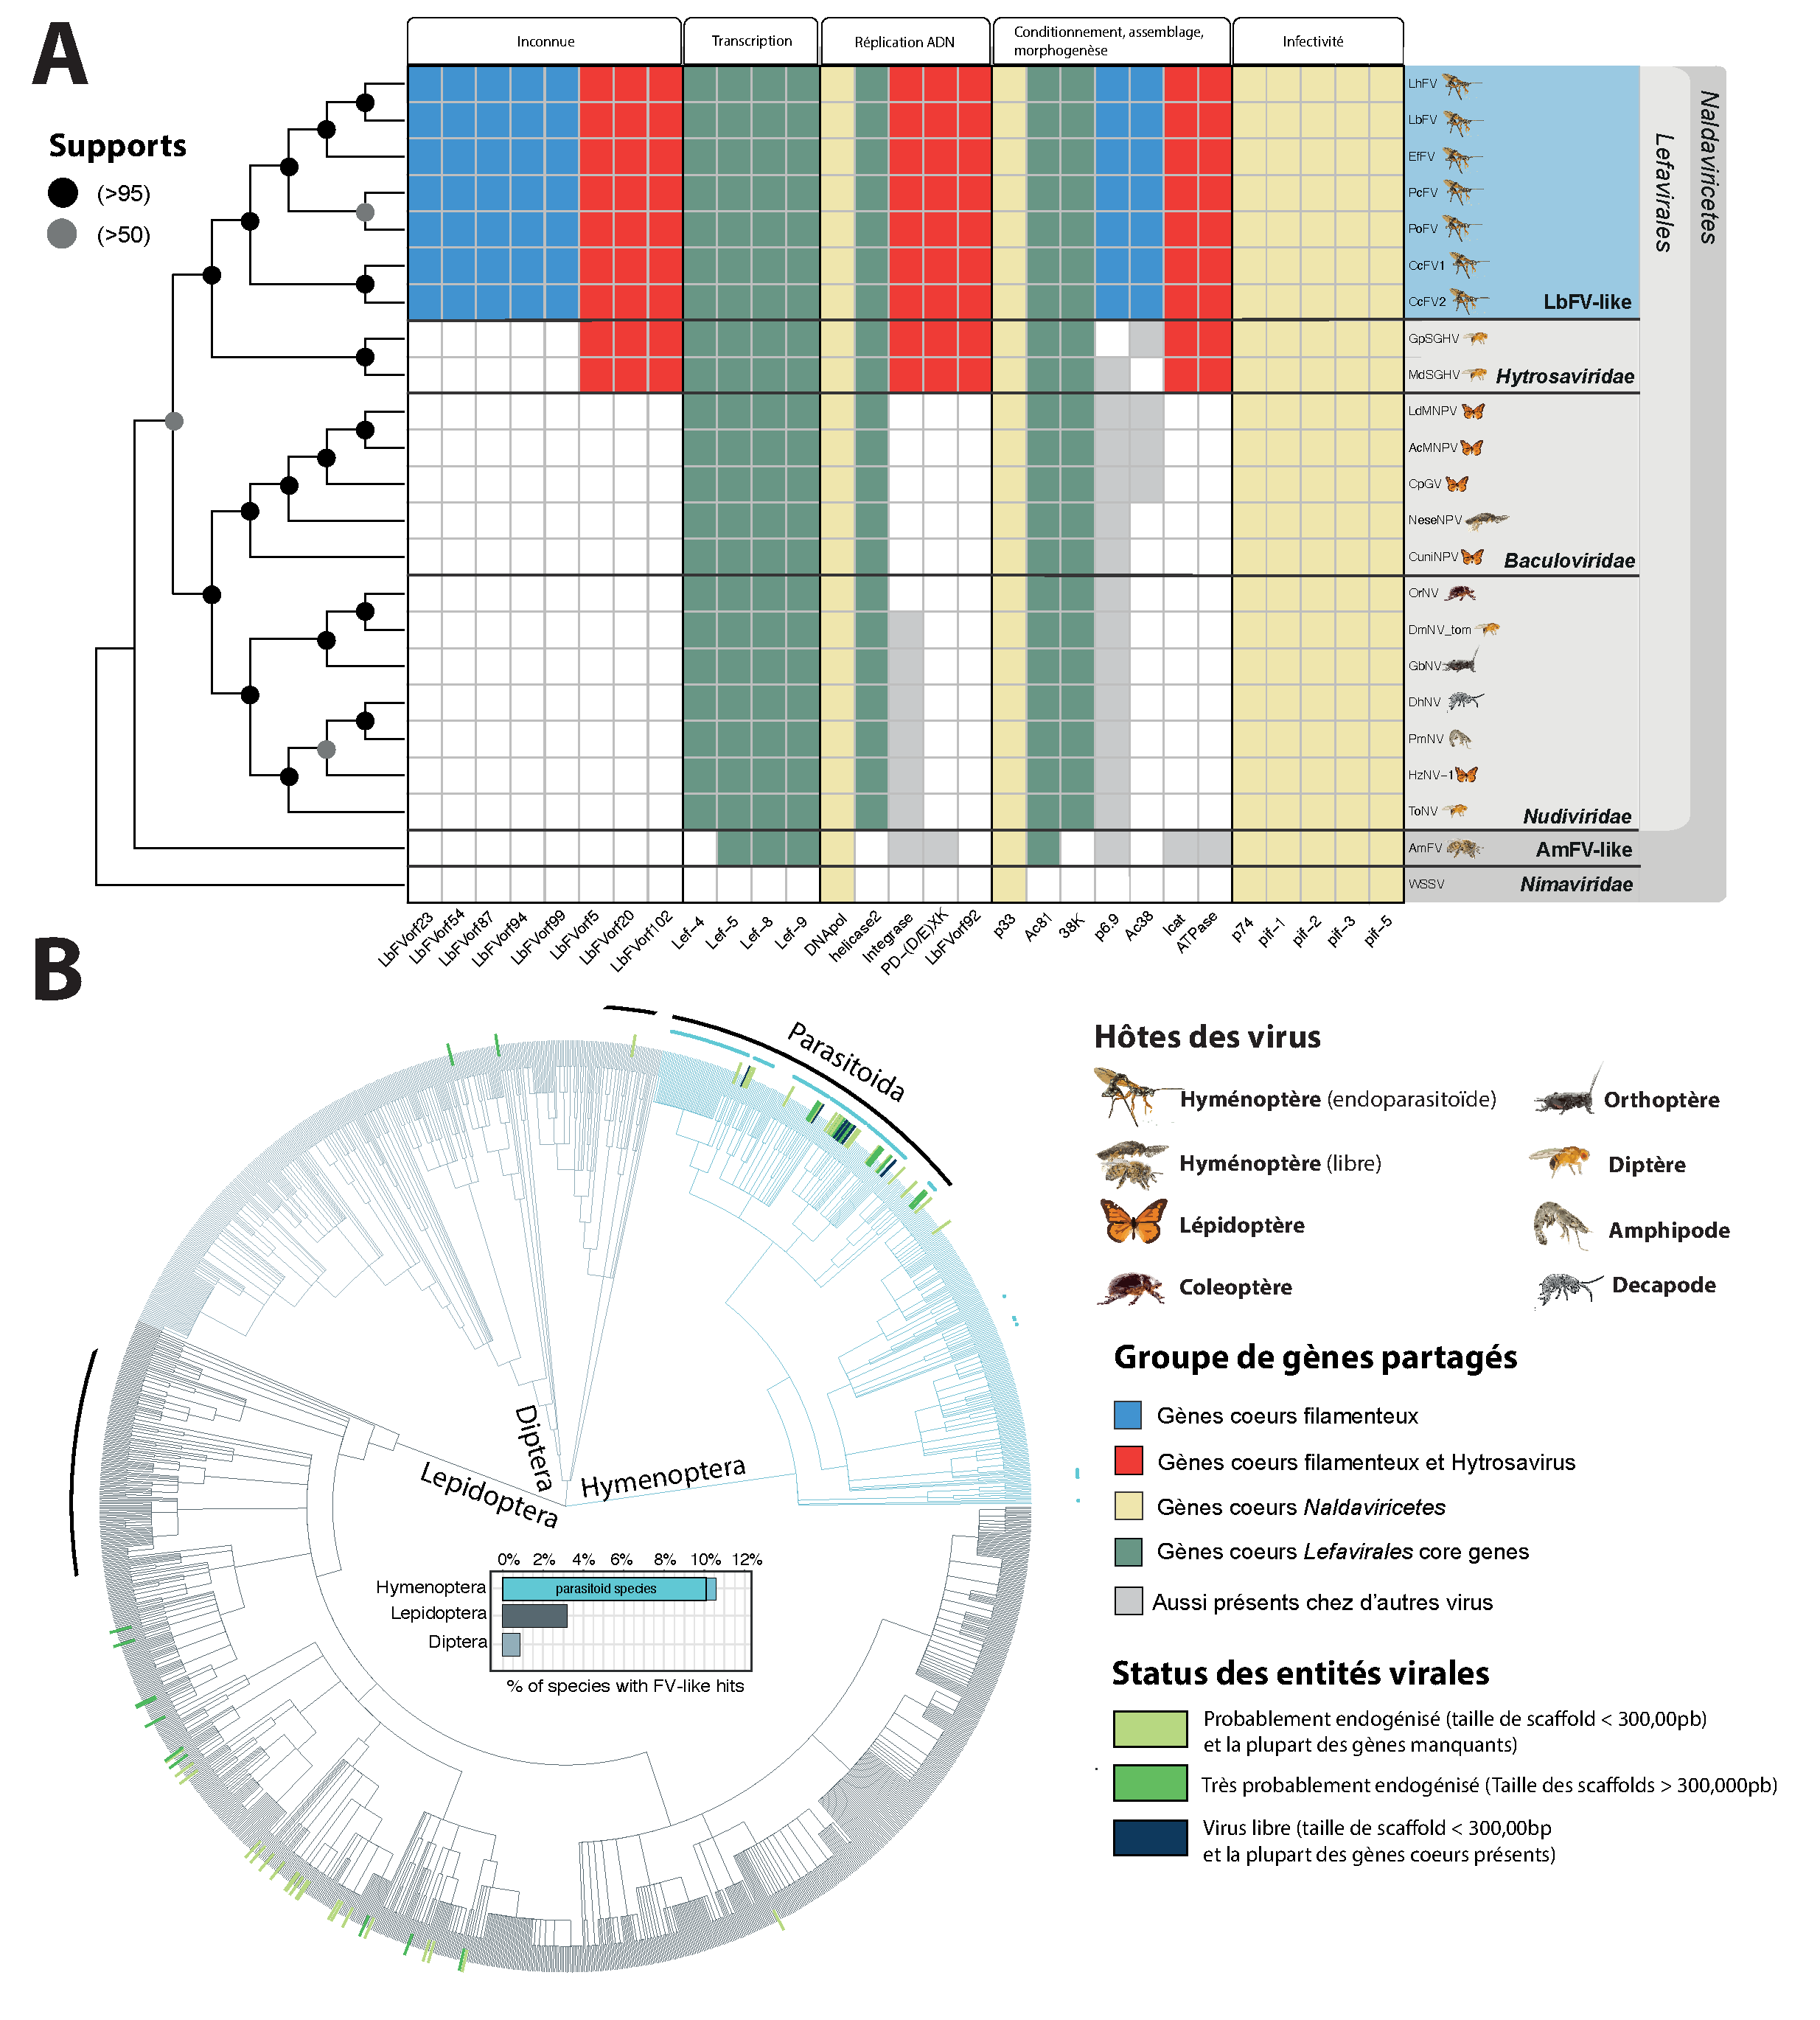
\includegraphics[width=\linewidth,height=\textheight,keepaspectratio]{PhD-master/figures/Resume_figure_papier2.pdf}
\caption[Paper2:Figures principales récapitulatives du chapitre2]{\footnotesize\textbf{Figures principales récapitulatives du chapitre2}. \textbf{A} - Heatmap représentant le contenu en gènes principaux des virus filamenteux par rapport aux autres espèces virales à ADNdb de la classe des \textit{Naldaviricetes}. Un cladogramme phylogénique est reporté sur la droite. Les lignes représentent les espèces virales, et les colonnes représentent les gènes distribués en fonction de leurs fonctions potentielles. Les cellules colorées représentent la présence du gène dans les génomes viraux (jaune pâle = gènes cœurs partagés par les espèces \textit{Naldaviricetes}, vert = gènes cœurs partagés par les espèces \textit{Lefavirales}, rouge = gènes cœurs filamenteux et hytrosavirus, bleu = gènes cœurs filamenteux et gris = présence dans d'autres génomes viraux). Les ordres des hôtes des virus sont affichés à côté du nom des virus. \textbf{B} - L'arbre phylogénétique circulaire montre les relations évolutives entre trois ordres d'insectes. La couleur des branches fait référence aux ordres d'insectes : bleu = Hyménoptères, gris clair = Diptères, gris foncé = Lépidoptères. Chaque tiret de couleur le long des feuilles de l'arbre représente le statut des éléments filamenteux (vert = FV endogène, bleu foncé = FV exogène vivant librement). Le cladogramme phylogénétique a été reconstruit sur la base du niveau NCBI taxonomique de tous les génomes étudiés dans cette analyse en utilisant la fonction NCBITaxa ete3 en python. La distribution du pourcentage d'espèces ayant des séquences de type FV dans chaque ordre d'insecte analysé est affichée dans le cladogramme à l'intérieur de la phylogénie.}
\label{figure:Resume_figure_papier2}
\end{figure}


Une propriété importante de ces virus est qu'ils semblent se répliquer uniquement chez des Hyménoptères parasitoïdes. En effet, tous les virus filamenteux dépistés jusqu'à présent sont hébergés par des espèces de guêpes endoparasitoïdes (\figurename{\ref{figure:Resume_figure_papier2}}-A). Néanmoins, nous ne pouvons pas exclure complètement le biais inhérent aux sujets de recherche de nos deux équipes, qui se sont principalement concentrées sur les Hyménoptères endoparasitoïdes. Aussi, j'ai mené une exploration systématique des assemblages de génomes obtenus pour 1576 espèces incluant des Diptères, Lépidoptères et Hyménoptères. Ce travail a révélé la présence de scaffolds appartenant probablement à des virus "libres" chez quelques Hyménoptères, mais aucun chez les Diptères ou les Lépidoptères. (\figurename{\ref{figure:Resume_figure_papier2}}-B). De plus, nous retrouvons une plus grande proportion d'EVEs filamenteux à l'intérieur de génome d'Hyménoptères par rapport aux deux autres ordres (\figurename{\ref{figure:Resume_figure_papier2}}-B). Malgré tout, nous parvenons également à observer en plus faible fréquence des EVEs filamenteux dans les génomes de  Diptères et Lépidoptères, ce qui suggère soit que des transferts puissent être médiés par les parasitoïdes vers leurs hôtes (\figurename{\ref{figure:Resume_figure_papier2}}-B), soit que des virus filamenteux se répliquent également chez ces espèces. De plus, un patron très marqué est apparu au sein des Hymenoptères. En effet, l'écrasante majorité des insertions virales détectées au sein de cet ordre concernait des Hyménoptères endoparasitoïdes (36/87), mais aucun ecto-parasitoïde (0/29) et seulement quelques espèces libres (4/210).\\

Aussi, le mode de vie des parasitoïdes, en particulier endo, pourrait représenter une niche écologique favorisant le maintien et la propagation de ces virus au sein des populations de guêpes. En effet, le style de vie endoparasitoïde pourrait faciliter la transmission de virus de manière verticale de la mère à la progéniture \citep{martinez_additional_2016}, dans la mesure où les femelles endoparasitoïdes injectent fréquemment des "fluides" dans leur hôte. De plus, ce mode de vie pourrait faciliter la transmission horizontale en condition de superparasitisme (partage d'un hôte par différents individus de la même espèce)\citep{varaldi_infectious_2003,coffman_viral_2022,stasiak_characteristics_2005}. De ce point de vue, la question qui reste complètement ouverte est de savoir si la manipulation du comportement est une caractéristique généralisée à tous les Filamentoviridae ou non. À ce propos, parmi 20 gènes de LbFV potentiellement impliqués dans la manipulation du comportement chez \textit{L.boulardi} \citep{varaldi_deciphering_2018}, 2 gènes font partie des 5 gènes cœurs spécifiques de la famille des Filamentoviridae. Ceci suggère que ces gènes pourraient être impliqués dans la modification comportementale de tous les Filamentoviridae. Il est clair cependant que des données phénotypiques supplémentaires et des essais fonctionnels avec d'autres guêpes infectées par des virus filamenteux seront nécessaires pour évaluer cette hypothèse.\\

En conclusion, ces résultats suggèrent que les virus filamenteux constituent une nouvelle famille préférentiellement associée au style de vie parasitoïde et distincte des \textit{Hytrosaviridae} et nous permettent de proposer les Filamentoviridae comme quatrième famille de virus dans l'ordre des \textit{Lefavirales}, rejoignant les familles \textit{Hytrosaviridae}, \textit{Nudiviridae} et \textit{Baculoviridae}. Des recherches supplémentaires sont nécessaires pour étudier la relation entre ces virus et leurs hôtes parasitoïdes et pour acquérir une connaissance plus approfondie du rôle des virus filamenteux dans les interactions parasitoïdes-virus. \\

Ces travaux complets en anglais sont disponibles dans la deuxième section du chapitre \hyperref[sec:chap2]{Études}. 

